\documentclass{article}
\usepackage[utf8]{inputenc}
\usepackage{amsmath}
\usepackage{amssymb}
\usepackage{amsthm}
\usepackage{color}
\usepackage{mathtools}
\usepackage{blkarray}
\usepackage{tikz}
\usepackage{listings}
\usepackage{pgfplots }
\usepackage{xcolor}
\usepackage{enumitem}
\usepackage{tcolorbox}
\usepackage{float}
\usepackage{wasysym}
\usetikzlibrary{arrows}
\usepackage{graphicx}
\usepackage{hyperref}
\usepackage{ mathrsfs }
\usepackage{ textcomp }
\usepackage[a4paper, margin=1.2in]{geometry}


% General settings 
\newcommand{\courseid}{DM587}
\newcommand{\coursename}{Scientific Programming}
\newcommand{\papertitle}{Sheet 5}
\newcommand{\term}{Fall 2024}
\newcommand{\dept}{Department of Mathematics and Computer Science}


\newcommand{\en}[1]{\,\text{#1}}
\renewcommand{\t}[1]{\text{#1}}
\renewcommand{\inf}{\infty}

\usepackage{fancyhdr}
\usepackage{listings}
\lstset{language=c,
	basicstyle=\ttfamily\lst@ifdisplaystyle\footnotesize\fi,%\fontfamily{pzc}\selectfont,%
	stringstyle=\ttfamily,
	commentstyle=\ttfamily,
	showstringspaces=false,
	frame=lines, 
	breaklines=true, tabsize=2,
	extendedchars=true,inputencoding=utf8
}
%\lstavoidwhitepre

\makeatletter
\let\runauthor\@author
\let\runtitle\@title
\makeatother

\pagestyle{fancy}
\lhead{} 
\chead{{\sc \courseid{} -- \coursename }}
\rhead{}
\cfoot{Page \thepage}

\fancypagestyle{plain}{
	\lhead{%
		\dept\\
		University of Southern Denmark, Odense
	}
	\chead{}
	\rhead{%
		\today\\
		Marco Chiarandini
	}
	\lfoot{}
	\rfoot{}
	%\renewcommand{\headrulewidth}{0pt}
}

\title{\begin{flushleft}
		\vspace{-4ex}
		\courseid~--- \coursename \\[0.2cm]
		{\Large \papertitle, \term \\[0.2cm]}
%		{\large Author:	\authorname \\[3ex]}
		\hrule
		\vspace{-4ex}
	\end{flushleft}
}
\date{}

\begin{document}
\setlength{\baselineskip}{1.25\baselineskip} % sets line spacing to
% something which looks like 1.5.
\setlength{\parindent}{0em} % sets line spacing to something which looks like 1.5.
\maketitle


Exercises originally formulated by Daniel Merkel, solutions originally
prepared by {Robert Rasmussen}, former teacher and teaching assistant of
this course.


\section*{Exercise 1}
\begin{enumerate}[label = (\arabic*)]
	\item Extract the carbon backbone
	
	\begin{figure}[H]
		\centering
		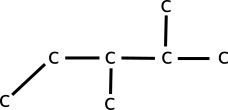
\includegraphics[width=0.4\textwidth]{exercise_1_1}
	\end{figure}
	
	Draw as a graph:

	\begin{figure}[H]
		\centering
		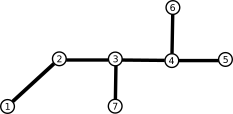
\includegraphics[width=0.4\textwidth]{exercise_1_2}
	\end{figure}
	
	Infer edge-weight matrix
	\[
		\begin{bmatrix}
			0 & 1 & \inf & \inf & \inf & \inf & \inf \\
			1 & 0 & 1 & \inf & \inf & \inf & \inf \\
			\inf & 1 & 0 & 1 & \inf & \inf & 1 \\
			\inf & \inf & 1 & 0 & 1 & 1 & \inf \\
			\inf & \inf & \inf & 1 & 0 & \inf & \inf \\
			\inf & \inf & \inf & 1 & \inf & 0 & \inf \\
			\inf & \inf & 1 & \inf & \inf & \inf & 0 \\
		\end{bmatrix}
	\]
	
	\item Compute distance matrix (to speed up we use repeated squaring)
	\[
		W^2 = W \odot W = 
		\begin{bmatrix}
		0 & 1 & 2 & \inf & \inf & \inf & \inf \\
		1 & 0 & 1 & 2 & \inf & \inf & 2 \\
		2 & 1 & 0 & 1 & 2 & 2 & 1 \\
		\inf & 2 & 1 & 0 & 1 & 1 & 2 \\
		\inf & \inf & 2 & 1 & 0 & 2 & \inf \\
		\inf & \inf & 2 & 1 & 2 & 0 & \inf \\
		\inf & 2 & 1 & 2 & \inf & \inf & 0 \\
		\end{bmatrix}
	\]	

	\[
		W^4 = W^2 \odot W^2 = 
		\begin{bmatrix}
		0 & 1 & 2 & 3 & 4 & 4 & 3 \\
		1 & 0 & 1 & 2 & 3 & 3 & 2 \\
		2 & 1 & 0 & 1 & 2 & 2 & 1 \\
		3 & 2 & 1 & 0 & 1 & 1 & 2 \\
		4 & 3 & 2 & 1 & 0 & 2 & 3 \\
		4 & 3 & 2 & 1 & 2 & 0 & 3 \\
		3 & 2 & 1 & 2 & 3 & 3 & 0 \\
		\end{bmatrix}
	\]
	We could continue, but the longest path in the graph is of length $4$ so $W^4 = W^5 = \dots$. Thus, $D = W^4$.
	
	%Another view would be that all entries has a concrete value so nothing would change by computing e.g. $W^5$, $W^6$, $\dots$. 
	
	\item The wiener index is 
	\[
		W(G) = \frac{1}{2}\sum_{i=1}^{n}\sum_{j=1}^{n} D_{ij} = 46 
	\]
	(the sum of all entries in the upper triangle of $D$)
	
	\item Looking at the upper (or lower) triangular part of the distance matrix and count the occurrences of $3$, we find the number of shortest paths of length $3$. \\
	
	There are $6$ shortest paths of length $3$. 
	
	\item The value of $p_0$ is 
	\[
		p_0 = n - 3 = 4
	\]
	and the value of $w_0$ is 
	\[
		w_0 = \frac{1}{6}(n+1)n(n-1) = \frac{1}{6}\cdot 8\cdot 7\cdot 6 = 56
	\]
	where $n=7$ (number of carbon atoms/vertices). 
	
	\item The value of $t_0$ is
	\[
		t_0 = 745.42\cdot \log_{10}(n+4.4) - 689.4 = 98.44
	\]
	
	The value of $t_B$ (estimated boiling point) is
	\[
		t_B = t_0 - \left(\frac{98}{n^2}\cdot \left(w_0-W(G)\right)+5.5\cdot(p_0-p)\right) = 89.44^\circ C
	\]
	(again, $n=7$ (number of carbon atoms/vertices))\\
	
	The real boiling point is $89.7^\circ C$ according to a wikipedia search, ie. it is fairly close to the predicted value.
	
	
	\item The worst case performance for finding the distance matrix based on repeated squaring is $O(n^3\log n)$. Each modified matrix-matrix multiplication take $O(n^3)$ time and we perform $\log_2 n$ matrix-matrix multiplications.
	
	\item You could use the Floyd-Warshall algorithm (solves all-pairs shortest distance problem) with asymptotic worst case performance $O(n^3)$.\\
	
	%\noindent Loose thought: You could probably also change Strassen's algorithm to accommodate the modified matrix-matrix multiplication. This would give worst case performance $O(n^{\log_2 7}\cdot \log n)$.

	\noindent Remark: Knowledge about the Floyd-Warshall algorithm
        comes from course DM507, Algorithms and Data Structures.
\end{enumerate}

\section*{Exercise 2}

\begin{enumerate}[label = (\arabic*)]
	\item They can be used to obtain updated coordinates when $(x_1, y_1)$, $(x_2, y_2)$, $\dots$, $(x_n, y_n)$ are represented as vectors in $\mathbb{R}^n$:
	\[
		\begin{bmatrix}
			x_1 \\ x_2 \\ \vdots \\ x_n
		\end{bmatrix} \ \ \ \ \ \ \ 
		\begin{bmatrix}
		y_1 \\ y_2 \\ \vdots \\ y_n
		\end{bmatrix}
	\]
	The update computes midpoints between connected points.	 

	\item Only $M_3$ is invertible (see \cite[p.~25]{random_polygon} or next sub-exercises)
	
	\item The determinants are
	\[
		\det(M_3) = \begin{vmatrix}
		1 & 1 & 0 \\
		0 & 1 & 1 \\
		1 & 0 & 1 
		\end{vmatrix} = 0.25 \ \ \ \ \text{(invertible)}
	\]
	and 
	\[
		\det(M_4) = \begin{vmatrix}
		1 & 1 & 0 & 0 \\
		0 & 1 & 1 & 0 \\
		0 & 0 & 1 & 1 \\
		1 & 0 & 0 & 1
		\end{vmatrix} = 0 \ \ \ \ \text{(not invertible)}
	\]
	
	\item 
	\begin{itemize}
		\item $M_3$: Yes - follows from Theorem 4.8.4 \cite[p.~228]{anton}.
		\item $M_4$: No - follows from Theorem 4.8.4 \cite[p.~228]{anton}.
		
		Note: Since the $4^{th}$ column is a linear combination of the others
		\[
			\begin{bmatrix}
			0 \\ 0 \\ 1 \\ 1
			\end{bmatrix} = 
			\begin{bmatrix}
			1 \\ 0 \\ 0 \\ 1
			\end{bmatrix} -
			\begin{bmatrix}
			1 \\ 1 \\ 0 \\ 0
			\end{bmatrix} +
			\begin{bmatrix}
			0 \\ 1 \\ 1 \\ 0
			\end{bmatrix}
		\]
		(see Theorem 4.3.1 \cite[p.~189]{anton})
	\end{itemize}

	\item An informal proof goes as follows:
	\begin{itemize}
		\item Do cofactor expansion on first column and realize that only the terms involving the first row first column and last row first column matters. When computing the determinant of the submatrix, for the term involving first row first column we are looking at a triangular matrix. Likewise, we are looking at a triangular matrix when removing the last row first column. 
		\item Observe these sub-(triangular)-matrices always have non-zero values of the diagonal (namely, $\frac{1}{2}$ as each entry), so they determinant are non-zero and are the same for both submatrices.
		\item When $n$ is even, the two terms cancel each other out given a determinant of $0$ ($M_n$ is not invertible). When $n$ is odd, the two terms don't cancel each other out ($M_n$ is invertible). 
	\end{itemize}
	
	% Daniel: Induction not necessary (at least not for this). Just write matrix M_x up, and observe that there are non-zero entries of diagonal, and on entries right above diagonal, and in the one in the bottom left corner. If we in cofactor exspansion removes bottom left entry somehow, we will have something which very intuitively must be either upper or lower triangular. 
	
	\item Drawing an equilateral triangle with points $(x_1^k, y_1^k)$, $(x_2^k, y_2^k)$, and $(x_3^k, y_3^k)$, we can find unique points $(x_1^{k-1}, y_1^{k-1})$, $(x_2^{k-1}, y_2^{k-1})$, $(x_3^{k-1}, y_3^{k-1})$ s.t. $x^k = M_3\cdot x^{k-1}$ and $y^k = M_3\cdot y^{k-1}$. 
	
	Why? Since $M_3$ is invertible we know there are unique solutions to $x^k = M_3\cdot x^{k-1}$ and $y^k = M_3\cdot y^{k-1}$, namely, $x^{k-1} = M_3^{-1}\cdot x^{k}$ and $y^{k-1} = M_3^{-1}\cdot y^{k}$. See an illustration of the situation in Figure \ref{fig:ex_2_6}.
	\begin{figure}[H]
		\centering
		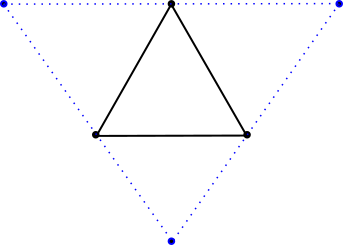
\includegraphics[width=0.5\textwidth]{exercise_2_6}
		%\caption{The black points are  $(x_1^k, y_1^k)$, $(x_2^k, y_2^k)$, and $(x_3^k, y_3^k)$. The blue points are $(x_1^{k-1}, y_1^{k-1})$, $(x_2^{k-1}, y_2^{k-1})$, $(x_3^{k-1}, y_3^{k-1})$.}
		\label{fig:ex_2_6}
	\end{figure}

	\item Drawing a square with points $(x_1^k, y_1^k)$, $(x_2^k, y_2^k)$, $(x_3^k, y_3^k)$, and $(x_4^k, y_4^k)$, we can find infinitely many points $(x_1^{k-1}, y_1^{k-1})$, $(x_2^{k-1}, y_2^{k-1})$, $(x_3^{k-1}, y_3^{k-1})$, and $(x_4^{k-1}, y_4^{k-1})$ s.t. $x^k = M_4\cdot x^{k-1}$ and $y^k = M_4\cdot y^{k-1}$. 
	
	Why? Solving the systems $x^k = M_4\cdot x^{k-1}$ and $y^k = M_4\cdot y^{k-1}$ can yield zero solutions, one unique solution, or infinitely many solutions for $x^{k-1}$ and $y^{k-1}$. Below we show two different set of four points leading to a square when the associated vectors $x^{k-1}$ and $y^{k-1}$ are multiplied by $M_4$. Therefore, there are infinitely many solutions.
	\begin{figure}[H]
		\centering
		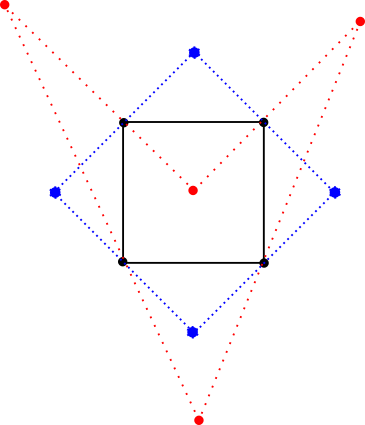
\includegraphics[width=0.5\textwidth]{exercise_2_7}
		%\caption{The black points are  $(x_1^k, y_1^k)$, $(x_2^k, y_2^k)$, and $(x_3^k, y_3^k)$. The blue (and red) points are $(x_1^{k-1}, y_1^{k-1})$, $(x_2^{k-1}, y_2^{k-1})$, $(x_3^{k-1}, y_3^{k-1})$.}
		\label{fig:ex_2_7}
	\end{figure}
	
			
	% Let consider a square with the points $(0,0)$, $(0,r)$, $(r,r)$, $(r,0)$ where $r$ is a positive real number. Solving the systems $x^k = M_4\cdot x^{k-1}$ and $y^k = M_4\cdot y^{k-1}$ yields solutions
	%\begin{align*}
	%	x^{k-1} & = \begin{bmatrix} -t+2r \\ t-2r \\ -t+2r \\ t\end{bmatrix}, \ \ t\in \mathbb{R}\\
	%	y^{k-1} & = \begin{bmatrix} -s \\ s \\ -s+2r \\ s \end{bmatrix}, \ \ s\in \mathbb{R}
	%\end{align*}
	%As we can see there are infinitely many solutions for $x^{k-1}$ and $y^{k-1}$. In short, the non-existence of an inverse of $M_4$ imply that we can't find unique points for $(x_1^{k-1}, y_1^{k-1})$, $(x_2^{k-1}, y_2^{k-1})$, $(x_3^{k-1}, y_3^{k-1})$, and $(x_4^{k-1}, y_4^{k-1})$.
	%Note: It easy to illustrate the situation using \href{https://www.geogebra.org/classic}{GeoGebra}.
	
\end{enumerate}

\section*{Exercise 3}


\begin{enumerate}[label = (\arabic*)]
	\item The average of $v$ is
	\[
		\frac{0 + 3 + (-1) + 11 + (-3)}{5} = 2
	\]
	and thus $\bar{v}$ is
	\[
		\bar{v} = \begin{bmatrix}
		2 \\ 2 \\ 2 \\ 2 \\ 2
		\end{bmatrix}
	\]
	
	The value of $w$ is
	\[
		w = v - \bar{v} = \bar{v} = \begin{bmatrix}
		0 \\ 3 \\ -1 \\ 11 \\ -3
		\end{bmatrix} - \begin{bmatrix}
		2 \\ 2 \\ 2 \\ 2 \\ 2
		\end{bmatrix} = 
		\begin{bmatrix}
		-2 \\ 1 \\ -3 \\ 9 \\ -5
		\end{bmatrix}
	\]
	
	Remark: The mean of $w$ is $0$. To prove that the mean of $w = v-\overline{v}$, where $\overline{v}$ is a vector where each entry is the mean of all values $v_i$, is $0$ for an arbitrary vector $v\in \mathbb{R}^n$, do the following. Let $m$ be the average of the entries of $v$. Observe the mean of the entries of $w$ is
	\begin{align*}
		\frac{w_1 + w_2 + \dots + w_n}{n} & = \frac{(v_1 - m) + (v_2 - m)  + \dots + (v_n - m)}{n} \\
		& = \frac{(v_1 + v_2 + \dots + v_n) - n\cdot m}{n} \\
		& = \frac{(v_1 + v_2 + \dots + v_n)}{n} - \frac{n\cdot m}{n} \\
		& = m - m \\
		& = 0
	\end{align*}
	
	\item Normalizing $w$ gives 
	\[
		\frac{w}{||w||_2} = \frac{1}{\sqrt{(-2)^2 + 1^2 + (-3)^2 + 9^2 + (-5)^2}}\begin{bmatrix}
		-2 \\ 1 \\ -3 \\ 9 \\ -5
		\end{bmatrix} = \frac{1}{\sqrt{120}} \begin{bmatrix}
		-2 \\ 1 \\ -3 \\ 9 \\ -5
		\end{bmatrix}
		= \begin{bmatrix}
		-\frac{2}{\sqrt{120}} \\ \frac{1}{\sqrt{120}} \\ -\frac{3}{\sqrt{120}} \\ \frac{9}{\sqrt{120}} \\ -\frac{5}{\sqrt{120}}
		\end{bmatrix}
	\]
	
	\item The lenght of $\frac{w}{||w||_2}$ is
	\[
		\left|\left|\frac{w}{||w||_2}\right|\right| = \sqrt{\left(-\frac{2}{\sqrt{120}}\right)^2+\left(\frac{1}{\sqrt{120}}\right)^2+\left(-\frac{3}{\sqrt{120}}\right)^2+\left(\frac{9}{\sqrt{120}}\right)^2+\left(-\frac{5}{\sqrt{120}}\right)^2} = 1
	\]
	
	
\end{enumerate}

\section*{Exercise 4}
\begin{enumerate}[label = (\arabic*)]
	\item Just do it!
	\begin{lstlisting}
	In [1]: 0.1+0.2
	Out[1]: 0.30000000000000004
	\end{lstlisting}
	
	See
        \url{https://docs.python.org/3.6/tutorial/floatingpoint.html}
        and \cite[p.~377]{stallings} for an explanation.
	
	\item 
	
	\begin{enumerate}[label = (\alph*)]
		\item In all cases we except the same result mathematically, namely, that $c = a$ is true.
		
		\item I guess all of them.
		
		The obvious problem with (a) is $a$ at some point will become closer to the representation of $0$. When this occurs, no matter how many times you multiply $a$ by $2$, $a$ will always remain $0$.
		
		In (b), adding $1$ after each division is introduced; thereby, the $0$-problem from (a) is removed. However, at some point $a$ will get to close to $2$; thus, the second for-loop just subtracts $1$ from $2$ and multiplies the result by $2$ obtaining $2$ again.
		
		In (c), adding $10000$ after each division also removes the $0$-problem from (a), however, a similar problem to (b) is that $a$ becomes increasingly close to $20000$. If $a$ becomes $20000$, then subtracting $10000$ from $20000$ and multiplying by $2$ just gives $20000$ again. 
		
		\item In (a) the value of $c$ should be high since it should have been exposed to a lot of division.
		
		In (b), the value of $c$ should also be relatively high (however less than in (a)). %(however less than in (a) since the possible values gets closer near $0$ and father apart when moving away \cite[p.~377]{stallings})
		
		In (c), the value of $c$ should be around the same as for (b) (maybe a bit less) before creating a numerical issue.
		
		\item Since as observed in \cite[p.~26-27]{random_polygon}, numerical issues occur in our approach to the "From Random Polygon to Ellipse” problem, and therefore we should be aware of it. 
	\end{enumerate}
\end{enumerate}


\clearpage
\bibliography{sources}
\bibliographystyle{plain}


\end{document}
